\subsection[Bootstrap et CSS]{\bs{} \& \css{}}
\subsubsection[Qu'est-ce que le CSS?][fr.wikipedia.org/wiki/Feuilles\_de\_style\_en\_cascade]{Qu'est-ce que le \css{}?}\label{sec:css} 
\textit{``De la même façon que HTML, CSS\footnote{Cascading Style Sheets} n'est pas vraiment un langage de programmation. C'est un langage de feuille de style, c'est-à-dire qu'il permet d'appliquer des styles sur différents éléments sélectionnés dans un document HTML''.} (\href{https://developer.mozilla.org/fr/docs/Learn/Getting_started_with_the_web/CSS_basics}{developer.mozilla.org}). Cela signifie que le \css{} est le langage utilisé pour décrire comment chaque élément \html{} doit être affiché. Cela va de la taille et couleur du texte à la création de \verb|navbar|, \verb|buttons|, \verb|tables|, etc\ldots en passant par diverses animations simples ou plus complexes.

Le langage suit la philosophie suivante: à chaque sélecteur, on associe des propriétés. Les sélecteurs peuvent être des tags \html{} eux-mêmes, des \verb|class|, \verb|id|, ou d'autres choses. La bonne pratique est de styliser un maximum de composants en créant une multitude de \verb|class| ayant chacune une tâche spécifique (taille, couleur, etc) afin d'obtenir une structure générale et modulaire, et ensuite d'assigner autant de \verb|class| que l'on veut aux tags \html{} que l'on souhaite modifier. Plus de détails dans la section dédiée (WIP).

\subsubsection[A quoi sert Bootstrap?][fr.wikipedia.org/wiki/Bootstrap\_(framework)]{A quoi sert \bs{}?}
Autant dire que la philosophie décrite conduit très rapidement à des fichiers énormes (milliers de lignes), illisibles, de successions de sélecteurs$\rightarrow$propriétés, ce qui conduit à une maintenance plus que laborieuse, alors que là n'est souvent pas la partie sur laquelle les développeurs veulent passer du temps (sauf si c'est leur métier, évidement\footnote{on parle alors de développeurs \textit{front-end}, responsables entre autres du rendu des sites.}). C'est pour cela que de nombreux \textit{frameworks front-end} existent afin d'amener de nombreuses \verb|class| et plugins \js{} prédéfinis. En l'occurence, nous allons utiliser \bs{}, qui est un \textit{framework} utilisé pour construire des sites de manière \textit{responsive\footnote{\textit{responsive} signifie que le site/composant adapte son rendu en fonction de la taille de l'écran, du format etc, ce qui est quand même très important.}} rapidement et facilement.

Pour plus de renseignement et pour découvrir les fonctionnalités de \bs{}, rendez-vous sur \href{https://getbootstrap.com/docs/5.3/getting-started/introduction/}{Doc \bs{}}. Dans la \texttt{Section (WIP)} et dans votre futur, vous utiliserez énormément de \verb|class| \bs. Il est donc imporant de se familiariser avec rapidement, par exemple en lisant la documentation des \verb|class| que vous ne connaissez pas, même si c'est fort déroutant au début afin que cela roule tout seul à moyen terme.

\subsubsection[Vite][laravel.com/docs/10.x/vite\#introduction]{\vite{}? Comme la rapidité de cette formation?}
Les \textit{frameworks} ``règlent le problème'' des 10000 lignes de code à écrire, mais pas celui de leur gestion et compilation. Rentre alors en scène \vite:

\textit{``Vite is a modern frontend build tool that provides an extremely fast development environment and bundles your code for production\footnote{\textit{production} signifie le déploiement du site pour le public}. When building applications with Laravel, you will typically use Vite to bundle your application's CSS and JavaScript files into production ready assets''.} (\href{https://laravel.com/docs/10.x/vite#introduction}{Doc \laravel{}}).

\subsubsection[Installation]{Installation}

Pour installer \bs{}, il suffit d'exécuter les commandes suivantes:
\begin{enumerate}
    \item \verb|sail npm install bootstrap @popperjs/core|, qui permet d'installer \verb|Popper|, une bibliothèque \js{} utilisé par \bs{}.
    \item \verb|sail npm install sass --save-dev|, qui permet d'utiliser le langage \sass{}, utilisé par \\ \bs{}.
\end{enumerate}

\begin{wrapfigure}{r}{0.3\textwidth}
    \vspace{-0.5cm}
    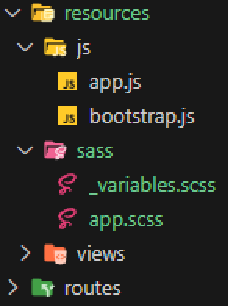
\includegraphics[width=0.25\textwidth]{figures-C1/bs_setup.pdf}
    \caption{\label{fig:bs_setup}}
\end{wrapfigure}
Ensuite, dans le dossier \verb|resources|, nous allons renommer le dossier \verb|css| en \verb|sass| et le fichier \verb|app.css| à l'intérieur en un fichier \verb|app.scss|. Il nous reste ensuite à ajouter un fichier \verb|_variables.scss| dans le dossier \verb|sass|, que nous utiliserons plus tard. Pour l'instant, nous allons juste le remplir avec le contenu de la \textsc{Figure~\ref{fig:variables.scss}}. Vous devriez donc obtenir un arrangement comme à la \textsc{Figure~\ref{fig:bs_setup}}. Comme nous le verrons à la \textsc{Figure~\ref{fig:vite_config}}, le fichier \verb|app.scss| est compilé par \vite{} en un fichier \css{} dans le dossier \verb|public| qui permettra de custommiser notre site web. Il faut donc le remplir par ce qui est donné par la \textsc{Figure }\ref{fig:app.scss}, où la première ligne permet de changer la police d'écriture utilisée par défaut (avec celle ajoutée dans \verb|_variables.scss|), la deuxième importe le fichier \verb|variables.scss| que nous venons de créer (qui pour le moment est vide) et enfin la troisième importe toutes les fonctionnalités de \bs{}. Nous verrons dans une future section (WIP) comment personnaliser ces importations pour n'importer que les fonctionnalités que l'on utilise, et donc gagner en performances. 

Par ailleurs, lorsque nous créerons des codes \sass{} custom, nous les utiliserons en les importants dans le fichier \verb|app.scss|.

\begin{figure}[!h]
    \begin{minipage}{0.44\textwidth}
        \centering
        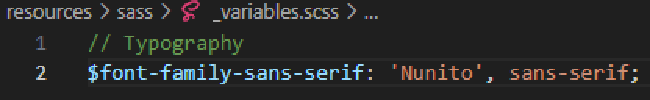
\includegraphics[width=\textwidth]{figures-C1/variables.pdf}
        \caption{\label{fig:variables.scss}}
    \end{minipage} 
    \begin{minipage}{0.54\textwidth}
        \centering
        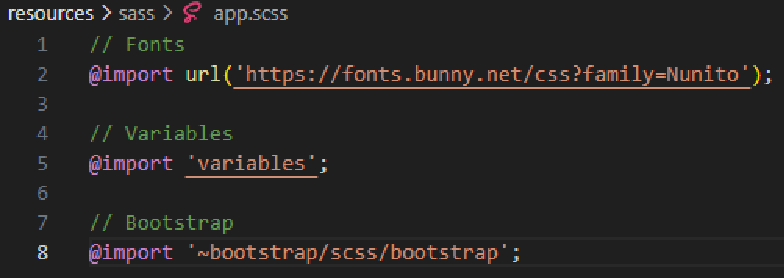
\includegraphics[width=\textwidth]{figures-C1/app.scss.pdf}
        \caption{\label{fig:app.scss}}
    \end{minipage}
\end{figure}

En ce qui concerne le code \js{} utilisé par \bs{}, il faut l'importer en ajoutant \verb|import * as bootstrap from 'bootstrap'| dans le fichier \verb|resources/js/app.js|.
\newpage

\begin{wrapfigure}[12]{r}{0.65\textwidth}
    \vspace{-0.5cm}
    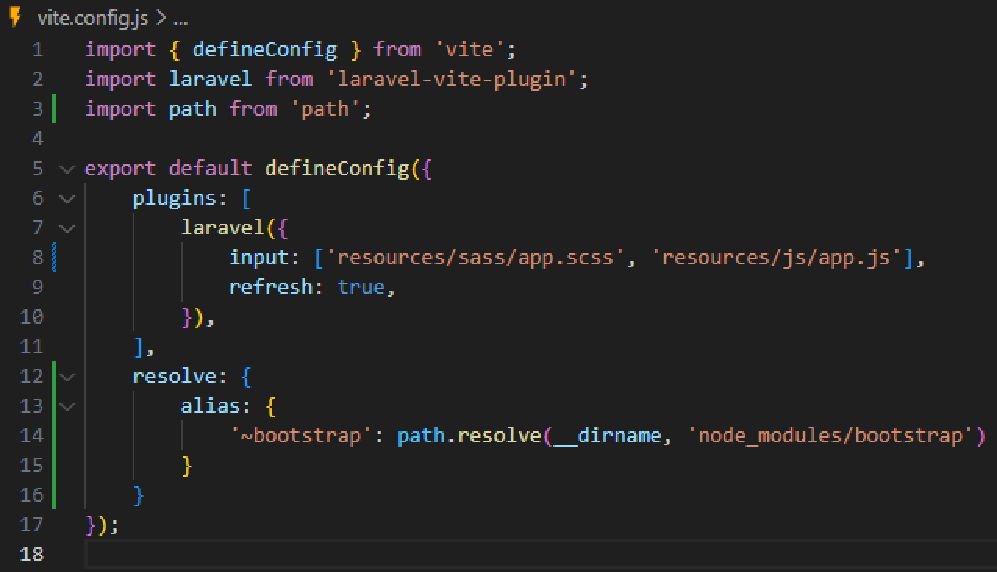
\includegraphics[width=0.65\textwidth]{figures-C1/vite.config.pdf}
    \caption{\label{fig:vite_config}}
\end{wrapfigure}

Enfin, il faut modifier les paramètres de \vite{} pour prendre en compte les changements que nous avons mis en place. Modifier donc la ligne 8 et ajoutez d'autres lignes dans le fichier \verb|vite.config.js| situé dans le dossier racine du site.

\underline{PS:} Si vous utilisez WSL2, vous avez normalement un bout de code en plus dans ce fichier, il faut bien évidement le laisser.

\vspace{0.3cm}

\begin{wrapfigure}[11]{r}{0.65\textwidth}
    \vspace{-0.5cm}
    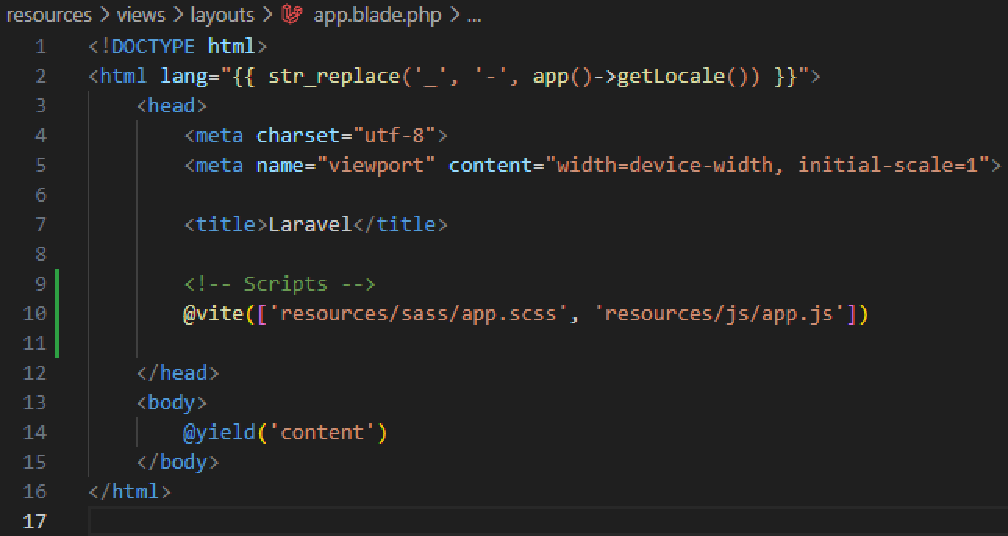
\includegraphics[width=0.65\textwidth]{figures-C1/vite_in_layout.pdf}
    \caption{}
\end{wrapfigure}

Remarquez que jusqu'ici, on ne voit toujours pas de changement quand on va sur notre site. La raison est que nous n'avons pas encore ``dit'' à nos \views{} d'utiliser nos ajouts. Pour cela, rendez-vous dans notre layout (càd \verb|app.blade.php|) et ajoutons la ligne suivante:

\vspace{1cm}
Maintenant, tout est prêt pour commencer à utiliser \bs{}.

\subsubsection[Utilisation]{Utilisation}

Comme expliqué plus haut, \bs{} nous fournit une multitude de \verb|class| que nous pouvons utiliser pour styliser nos \textit{tags} \html{}. Modifions donc nos \views{} \verb|about.blade.php| et \verb|index.blade.php| comme aux \textsc{Figures~\ref{fig:about_bs}\&\ref{fig:index_bs}}.

\SaveVerb{about}|about.blade.php|
\SaveVerb{index}|index.blade.php|
\begin{figure}[!ht]
    \centering
    \begin{minipage}{0.28\textwidth}
         \centering
         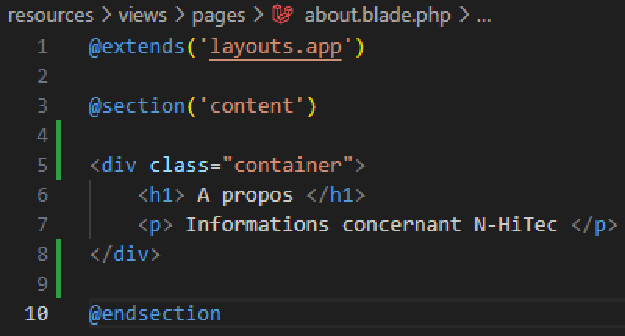
\includegraphics[width=\textwidth]{figures-C1/about_bs.pdf}
         \caption{\\\hspace{\textwidth} \protect\UseVerb{about}\label{fig:about_bs}}
    \end{minipage}
    \begin{minipage}{0.7\textwidth}
         \centering
         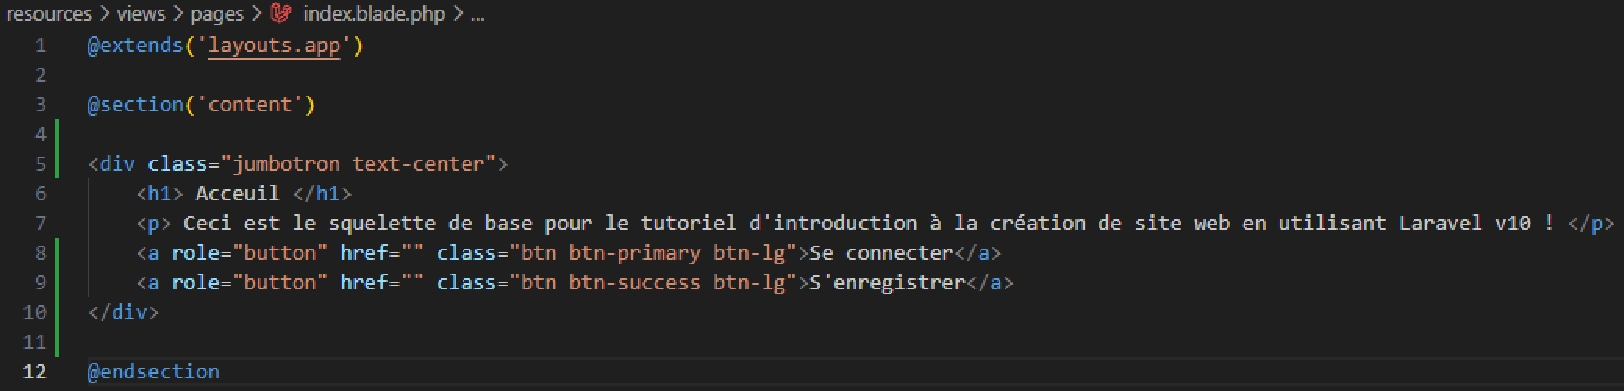
\includegraphics[width=\textwidth]{figures-C1/index_bs.pdf}
         \caption{\protect\UseVerb{index}\label{fig:index_bs}}
    \end{minipage}
\end{figure}

Par exemple, dans la \textsc{Figure~\ref{fig:index_bs}}, \verb|class="text-center"| assigne la classe \verb|text-center| à l'élément, et en maintenant la touche \textit{Ctl} enfoncée et en passant le curseur sur la classe, vous verrez une classe\footnote{Avec les bonnes extensions VS code en tt cas\ldots voir les extensions dans la section~(WIP)} permettant de centrer un'élément dans son conteneur.

\begin{wrapfigure}{r}{0.55\textwidth}
    \vspace{-0.5cm}
    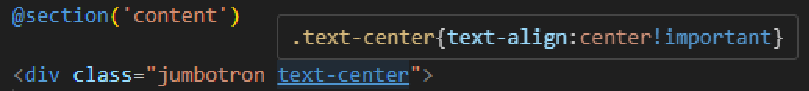
\includegraphics[width=0.55\textwidth]{figures-C1/see_class.pdf}
\end{wrapfigure}
Dans le petit cadre, nous voyons le code \css{}\footnote{voir \texttt{Section~\ref{sec:css}}} correspondant à cette classe.

Pour la customisation de la page des services, nous allons en profiter pour découvrir une nouvelle mécanique: passer des données aux pages. En effet, c'est quand même pratique de pouvoir afficher des informations dynamiquement! Pour le moment, nous n'allons pas encore s'embêter avec la base de donnée, nous allons juste voir comment la mécanique de base fonctionne. Rappelez-vous de la \texttt{Section~\ref{sec:fonctionnement&philosophie}}, ce sont les \controllers{} qui s'occupent de manipuler les données avant d'afficher une \view{}. Dès lors, c'est dans la fonction \verb|services()| de \verb|PagesController.php| que nous allons ajouter des choses:
\begin{figure}[!h]
    \centering
    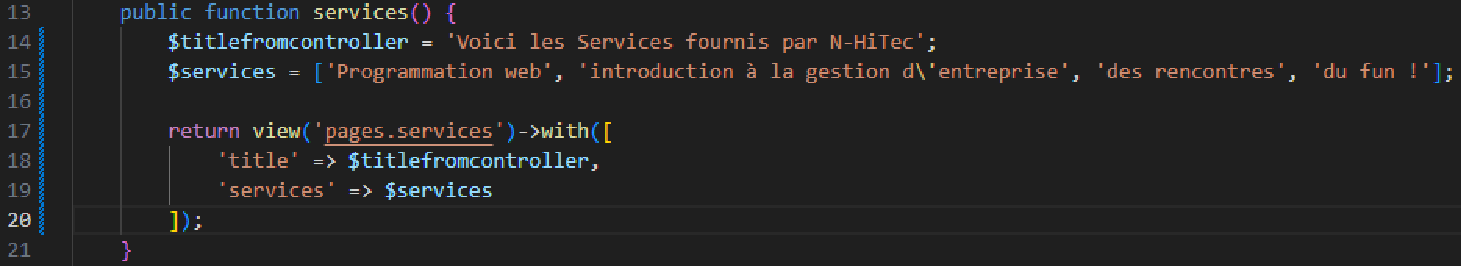
\includegraphics[width=\textwidth]{figures-C1/services_fct_bs.pdf}
    \caption{}
\end{figure}

\verb|$titlefromcontroller| et \verb|$services| sont 2 variables, et nous les passons à la \view{} par l'intermédiaire du \verb|->with(...)|. 

\begin{wrapfigure}[6]{r}{0.5\textwidth}
\vspace{-0.5cm}
    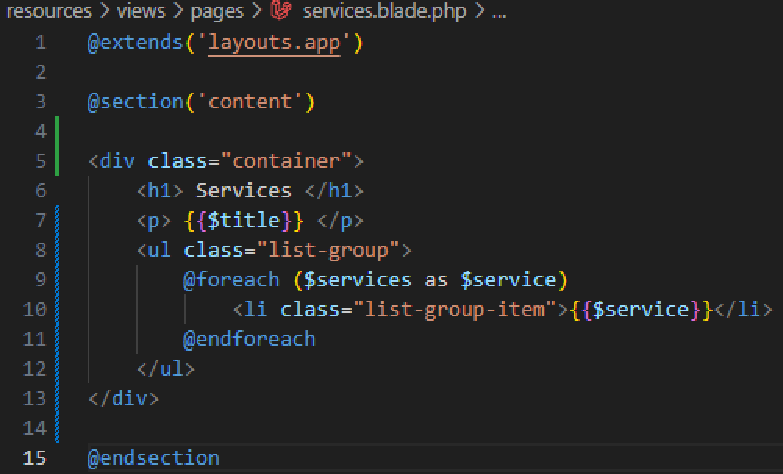
\includegraphics[width=0.5\textwidth]{figures-C1/services_bs.pdf}
    \caption{}
\end{wrapfigure}

Ensuite, nous pouvons utiliser les variables \verb|title| et \verb|services| dans la \view{} concernée. Dans la \texttt{Section~\ref{sec:welcome!}} nous avons pris connaissance des avantages du format \verb|.blade.php|. Celui-ci nous apporte donc les commandes \verb|{{}}|\footnote{Cette commande agit comme un \verb|printf()| en C. Elle permet d'afficher le contenu de la variable en argument.} et \verb|@foreach()|\footnote{Boucle \verb|foreach| classique, pour itérer sur un tableau. Les tags \verb|<a>| ainsi que \verb|<ul>| et \verb|<li>| seront expliqué à la section suivante.}.

\newpage

Et voilà! Maintenant, il suffit de taper \verb|sail npm run dev|\footnote{Cette commande permet de compiler le \css{} et \js{} en créant un mini serveur localement. Cette commande utilisée lors du \underline{DEVELOPPEMENT DU SITE} permet d'appliquer les modifications apportées à des fichiers rapidement sans devoir refresh la page. Pour compiler tout ça en production, il faut utiliser \verb|npm run build|. Plus de \verb|sail| car \laravelsail{} est un outil de développement, pas de déploiement!}(si ce n'était pas déjà fait) pour admirer le résultat. C'est déjà vachement mieux, non?

\begin{figure}[!h]
    \begin{subfigure}[c]{0.73\textwidth}
        \fbox{
\includegraphics[width=\textwidth]{figures-C1/web_index.pdf}}
    \end{subfigure}\hfill
    \begin{subfigure}[c]{0.24\textwidth}
        \caption{\url{http://tutorialstepbystep/}} 
    \end{subfigure}
    \begin{subfigure}[c]{0.73\textwidth}
        \fbox{
\includegraphics[width=\textwidth]{figures-C1/web_about.pdf}}
    \end{subfigure}\hfill
    \begin{subfigure}[c]{0.24\textwidth}
        \caption{\url{http://tutorialstepbystep/about}} 
    \end{subfigure}
    \begin{subfigure}[c]{0.73\textwidth}
        \fbox{
\includegraphics[width=\textwidth]{figures-C1/web_services.pdf}}
    \end{subfigure}\hfill
    \begin{subfigure}[c]{0.24\textwidth}
        \caption{\url{http://tutorialstepbystep/services}} 
    \end{subfigure}
    \caption{3 pages créées jusqu'à présent et stylisées avec \bs{}.}
\end{figure}
C'est bien beau, mais jusque ici le seul moyen de naviguer entre les pages est de rentrer leur URL, ce qui n'est ma foi pas fort pratique. Remédions à cela avant de passer à la suite.

\subsubsection[Navbar]{Navbar}

C'est un gros morceau qui utilise beaucoup des \verb|class| de \bs{}, donc il va falloir s'accrocher. D'abord, créez un dossier \verb|inc| dans \verb|resources/views| et un fichier \verb|navbar.blade.php| dans ce nouveau dossier. Remplissez ce fichier comme la \textsc{Figure~\ref{fig:navbar}}.

\begin{figure}[!h]
    \centering
    \begin{minipage}{0.7\textwidth}
         \centering
         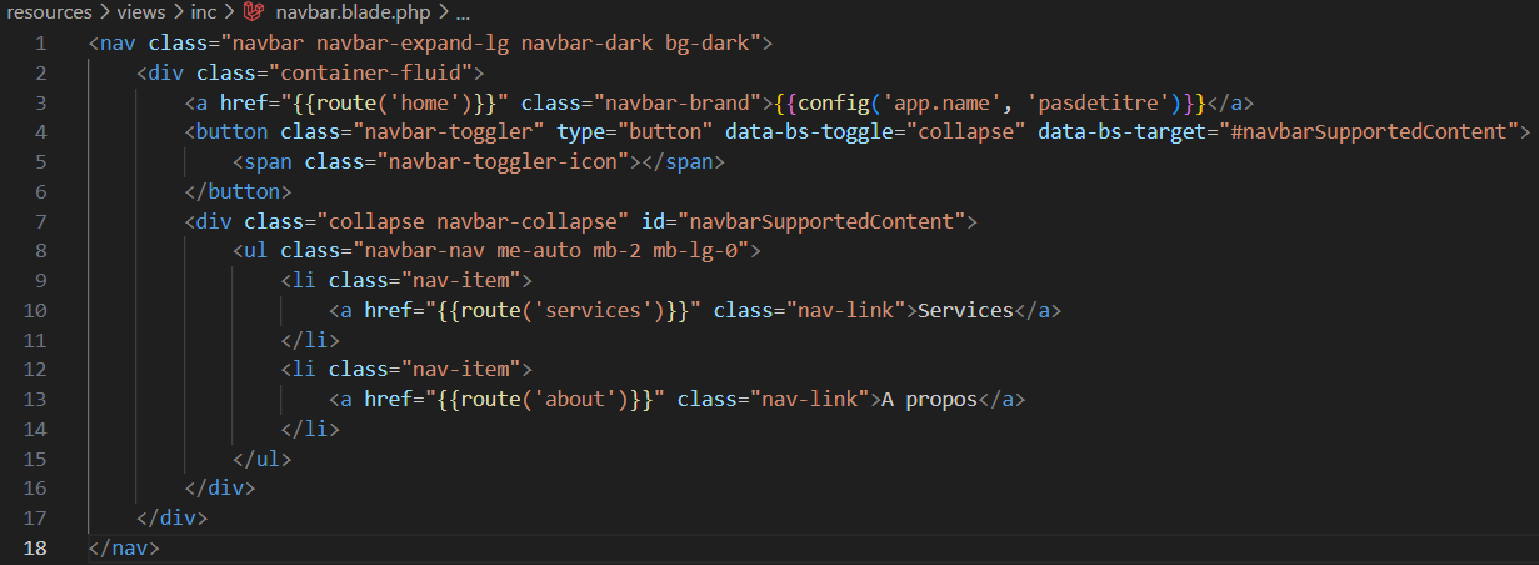
\includegraphics[width=\textwidth]{figures-C1/navbar.pdf}
         \caption{\label{fig:navbar}}
    \end{minipage}
    \begin{minipage}{0.28\textwidth}
         \centering
         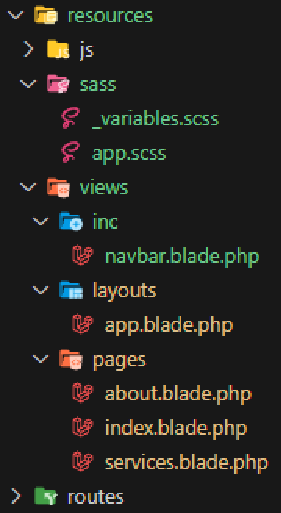
\includegraphics[width=0.5\textwidth]{figures-C1/navbar_file.pdf}
         \caption{}
    \end{minipage}
\end{figure}

\begin{wrapfigure}[2]{r}{0.3\textwidth}
    \vspace{-0.5cm}
    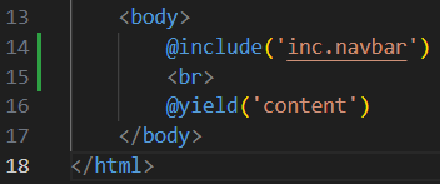
\includegraphics[width=0.3\textwidth]{figures-C1/navbar_layout.pdf}
\end{wrapfigure}

Ensuite, il faut ajouter notre \textit{navbar} à notre \textit{layout} afin qu'elle apparaisse sur toutes nos pages. Pour cela, rien de plus simple! 
\vspace{2cm}

\newpage

Qu'est ce que c'est que tout ça? Décomposons tout cela.
Premièrement, nous découvrons ici trois nouveaux tags \html{}:
\begin{enumerate}
    \item \verb|<a>| est un tag permettant la création d'un lien vers une autre URL, que l'on place dans l'attribut \verb|href|. Au lieu de tapez l'URL d'une \route{}, \laravel{} nous permet d'optimiser l'écriture en utilisant la commande \verb|route('nomdelaroute')| afin d'obtenir l'URL en question.~\verb|{{...}}| permet ensuite de l' ``afficher'' dans le \verb|href|.
    \item \verb|<ul>| est un tag signifiant la création d'une liste.
    \item \verb|<li>| représente un élément d'une liste.
\end{enumerate}

Pour le reste je vous invite à lire ce que font chaque \verb|class| et de jeter un oeil sur \href{https://getbootstrap.com/docs/5.3/components/navbar/}{la doc \bs{} sur les navbars}. Bien que ça soit indigeste lors d'une première lecture, ça l'est beaucoup moins que si nous devions analyser les \verb|class| une par une\ldots

Néanmoins, quelques notions clées: 
\begin{itemize}
    \item \textit{``collapsing''} fait référence au fait de faire disparaitre la navbar au profit d'une liste déroulable avec un bouton lorsque la largeur de l'écran devient plus petit qu'une valeure fixée (ici, $992\mathrm{px}$ car on utilise le mot clé \verb|lg|).
    \item le boutton spécial pour dérouler la navbar est créé par le tag \verb|<button class="navbar-toggler>|, qui est invisible lorsque la largeur de l'écran est > $992\mathrm{px}$.
    \item rien à voir avec \bs{}, \verb|config()| permet d'accéder à certaines valeurs, notament celles du \verb|.env|. En l'occurence, \verb|'app.name'| permet d'accéder à \verb|APP_NAME| (et si cette valeur n'existe pas, le deuxième argument est affiché).
\end{itemize}

Dans la \texttt{Section} (WIP), nous verrons comment améliorer cette navbar. En attendant, voilà ce à quoi elle devrait ressembler:

\begin{figure}[!h]
    \centering
    \begin{minipage}[b]{0.9\textwidth}
        \centering
        \fbox{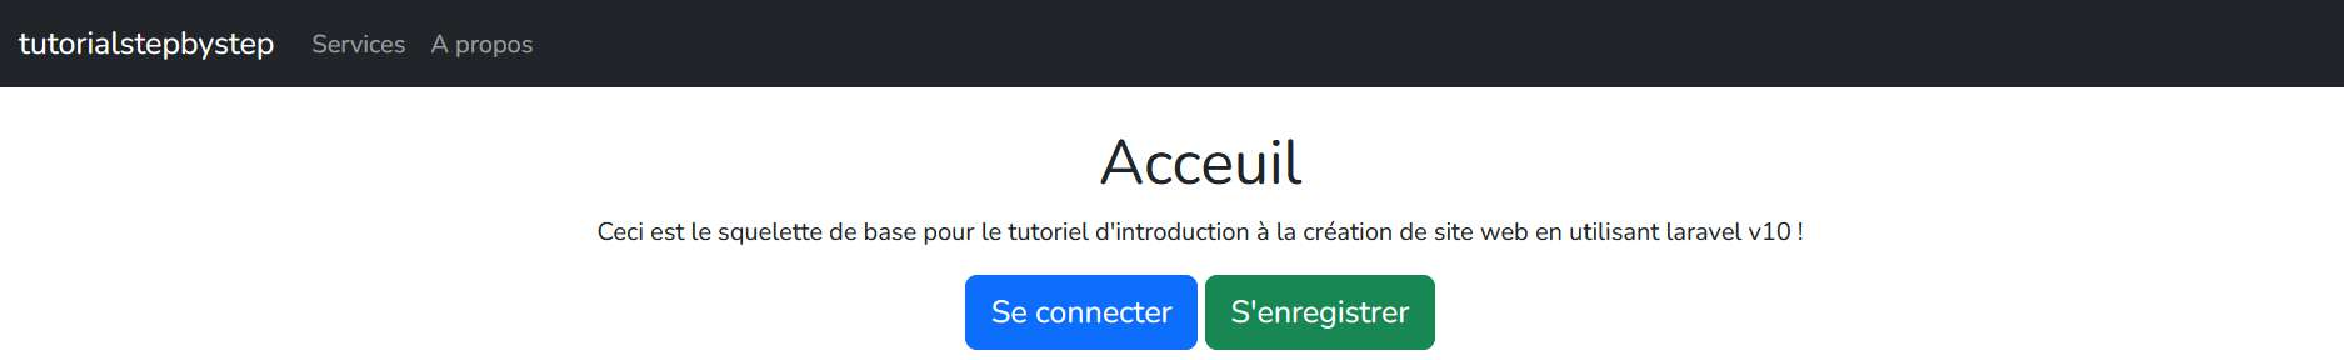
\includegraphics[width=\textwidth]{figures-C1/navbar_full.pdf}}
        \caption{navbar sur un écran de largeur $>992\mathrm{px}$}
    \end{minipage}
    \begin{minipage}[b]{0.44\textwidth}
        \centering
        \fbox{
\includegraphics[width=\textwidth]{figures-C1/navbar_full_phone_2.pdf}}
        \captionsetup{justification=centering}
        \captionof{figure}{navbar vue depuis un téléphone (largeur $<992\mathrm{px}$)}
    \end{minipage}
    \hspace{0.1cm}
    \begin{minipage}[b]{0.44\textwidth}
        \centering
        \fbox{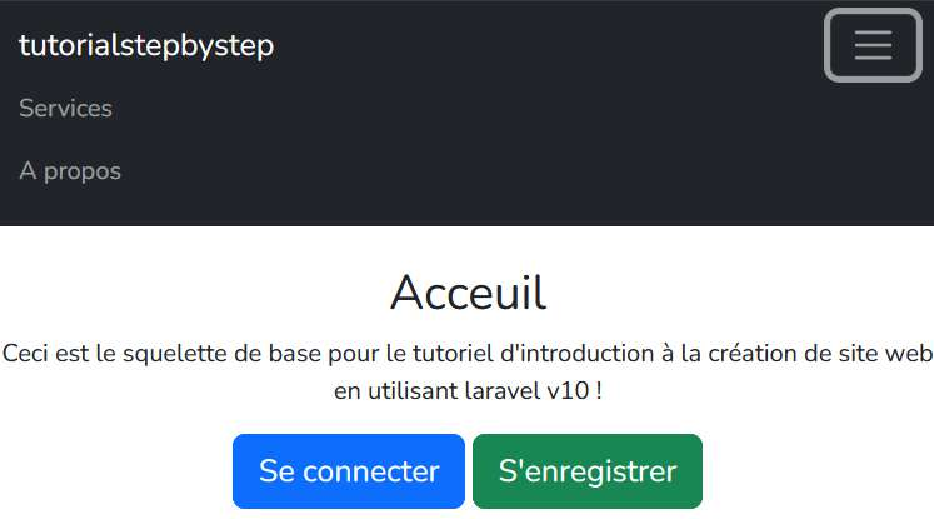
\includegraphics[width=\textwidth]{figures-C1/navbar_full_phone_1.pdf}}
        \captionsetup{justification=centering}
        \captionof{figure}{navbar en ayant appuyé sur le bouton en haut à droite}
    \end{minipage}
\end{figure}

\newpage
